\section{Call graph}
Sample code to call graph and then execution path, entry node, exit node.

\begin{figure}[h]	
	\centering
	\begin{subfigure}[h]{3in}
		%\centering
		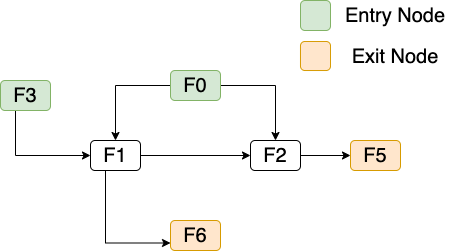
\includegraphics[width=3in]{figures/background/call graph.png}
		\caption{A sample call graph}\label{fig:agglomerative_clustering}		
	\end{subfigure}
	\quad
	\begin{subfigure}[h]{3in}
		%\centering
		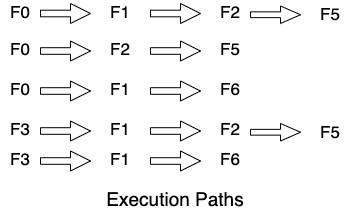
\includegraphics[width=3in]{figures/background/execution_paths.png}
		\caption{All execution paths from the call graph}\label{fig:1b}
	\end{subfigure}
	\caption{Call graph with entry node, exit node and execution paths}\label{fig:1}
\end{figure}

\section{Concept Cluster Tree}
Explain the concept cluster tree, with the role of leaf node, intermediate nodes for example. 
\section{Information Retrieval Techniques}
\subsection{TFIDF}
TFIDF is weight based statistical information retrieval technique. It tries to find important terms to a specific document by analyzing collection of documents. TFIDF is popular for document classification, search engine ranking and text mining\footnote{https://en.wikipedia.org/wiki/Tf–idf}. TFIDF ranks terms by term frequency-inverse document frequency score. Term frequency is count of a term in a document. Term frequency is biased towards common terms which mostly irrelevant to the document. 

\begin{equation}
    tf (W_x, D_x) = f_{W_x,D_x}
    \label{eq:tf_background}
\end{equation}
\begin{equation}
    idf(W_x) = \log(\frac{n}{df(W_x)})+1
    \label{eq:idf_background}
\end{equation}
\begin{equation}
    tf-idf(W_x, D_x) = tf(W_x,D_x) * idf(W_x)
    \label{eq:TFIDF_background}
\end{equation}


Jones \cite{jones1972statistical} introduced inverse document frequency which penalties common terms by counting their occurrence across the corpus. Let, $D = \{D_1, D_2, ..., D_n\}$ is a collection of documents and $W = \{W_1, W_2, ....., W_n\}$ is unique terms in the collection of documents. Now, to calculate term frequency for term $W_x$ in document $D_x$, we have to count frequency of term $W_x$ in  document $D_x$ which is required to calculate term frequency according to equation \ref{eq:tf_background}. In addition, we have to count the number of documents has term $W_x$ which is used to calculate inverse document frequency using equation \ref{eq:idf_background}. In equation \ref{eq:idf_background}, $n$ is the number of documents in the corpus and $df(W_x)$ is the number of documents which contain term $W_x$. Equation \ref{eq:TFIDF_background}, multiplies term frequency and inverse document frequency to reward significant terms and penalize common terms. 



\subsection{LSI}
Latent semantic indexing focuses on information retrieval based on semantic similarity between words where the previous techniques focus on matching words in query with words of documents. The semantic concept used in LSI assumes semantically similar words appear together. Information retrieval techniques which matches words suffer two limitations. They are \emph{synonymy} and \emph{polysemy}. \emph{synonymy} is the issue where same object is described by different words depending on needs, knowledge and linguistic habits. On the other hand, \emph{polysemy} is referred to the fact that words have multiple distinct meaning in different context. LSI, first, starts with Term-Document matrix where all terms are presented in the row and documents in the column. Table \ref{tb:LSI_term_document} shows an example of Term-Document matrix. 

\begin{table}[h]
    \centering
    \caption{Sample Term-Document matrix}
 \begin{tabular}{|c|c|c|c|c|c|c|}
    \hline
    
        & ship & boat & ocean & voyage & trip   \\
        \hline
        Document 1 & 1 & 0 & 1 & 0 & 0  \\
        Document 2 & 0 & 1 & 0 & 1 & 0    \\
        Document 3 & 1 & 0 & 0 & 1 & 1  \\
    \hline
    \end{tabular}
    
    \label{tb:LSI_term_document}
\end{table}


Term-Document matrix is projected to lower number of dimensions by Single Value Decomposition (SVD) method. The reduced matrix by SVD is approximation of the term-document matrix which is a representation of the semantic similarity between words in documents. If we need to find similarity between a query, the query is converted to similar representation and compared to find relevant documents. By using this technique, LSI can detect semantic similarity although the terms are different.   
\subsection{LDA}

\section{Jaccard Distance}
Jaccard Distance can measure similarity between two sequences according to equation \ref{eq:jaccard}. For example, we have two execution path $E_i$ and $E_j$ and they have set of function names $F_i$ and $F_j$ respectively. Therefore, similarity between $E_i$ and $E_j$ can be measured by equation \ref{eq:jaccard}. 
\begin{equation}
\label{eq:jaccard_similar}
    JD\_similar(E_i, E_j) =  \frac{F_i \bigcap F_j}{F_i \bigcup F_j}
\end{equation}

\begin{equation}
\label{eq:jaccard_dissimilar}
    JD\_dissimilar(E_i, E_j) =  1 - \frac{F_i \bigcap F_j}{F_i \bigcup F_j}
\end{equation}
If $E_i$ and $E_j$ are very similar, according to equation \ref{eq:jaccard_similar} similarity score will be near 1 and vice-versa. Clustering algorithm merges those two clusters which distance measures are minimum. Equation \ref{eq:jaccard_dissimilar} subtract Jaccard Distance by 1 to get desire dissimilarity measure for clustering algorithms.

\section{Agglomerative Hierarchical Clustering}
Clustering algorithms are popular in many data mining, unsupervised machine learning and pattern recognition applications. Clustering algorithm try to group similar observations together to find significant patterns in the observations. Hierarchical clustering can be done in two ways. One is bottom-up (agglomerative) and another is top-down (devisive). For Devisive clustering, all observations starts in a single cluster and divided into different clusters using heuristics. Agglomerative clustering starts by considering observations as individual clusters and then group them until all observations end-up in the same cluster.

\begin{figure*}[h]
  \centering
  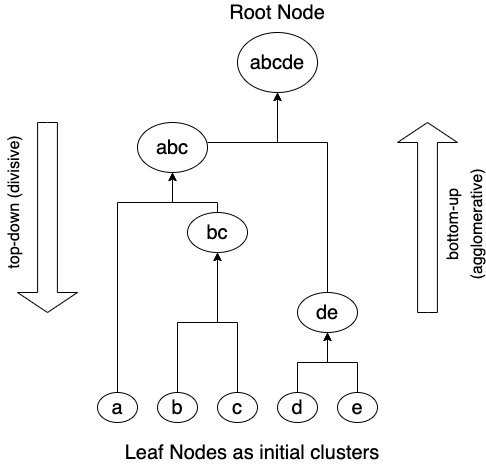
\includegraphics[width=0.5\columnwidth, height=0.5\columnwidth]{figures/background/agglomerative_clustering.png}
  \caption{Agglomerative and Divisive clustering algorithm with a sample cluster forest}~\label{fig:agglomerative_clustering}
\end{figure*}

\section{Text Rank}
Mihalcea \cite{mihalcea2004textrank} proposed graph based ranking algorithm inspired by PageRank algorithm to rank entities in natural language. Two of the significant application of TextRank are keyword extraction and sentence extraction. Sentence extraction can be formulated to generate summary of natural language text. To generate summary of a  text, first, sentences are split as they are the unit for TextRank algorithm. Next, sentences are converted to word embedding vectors. In the next step, similarity matrix is computed from embedding vectors. Then, a graph is created where vertices are sentences and edges represent similarity scores between sentences\footnote{https://www.analyticsvidhya.com/blog/2018/11/introduction-text-summarization-textrank-python/}. Similarity scores are used to extract top ranked sentences according to equation \ref{eq:textrank}.

\begin{equation}
\label{eq:textrank}
    WS(V_i) = (1 - d) + d * \sum_{V_j\epsilon IN(V_i) } \frac{w_{ji}}{\sum_{V_k \epsilon Out(V_j)} w_{jk}}  WS(V_j)
\end{equation}

Let, $ G = (V, E)$ is a directed graph where V is the collection of vertices and E is the collection of edges. $In(V_i)$ is the set of vertices which points to vertex $V_i$. Similarly, $Out(V_j)$ is the set of vertices which vertex $V_j$ points to. The similarity score between vertex $V_i$ and $V_j$ is represented by $w_{ji}$. 

\section{Pyramid Score}

\section{Sequential Pattern Mining}




